\chapter{Network from Text}

Now, let us try to generate networks from text. What do we mean by that? How can a text be transformed to a network? Well, documents are nodes, while edges can be the number of shared words. Again, we are back to similarity, but applied to text.

For this task, we will need the \emph{Text add-on}. Load \emph{grimm-tales-selected} with the \widget{Corpus} widget. This data set contains 44 Grimm's tales, some of which are tales of magic and some are animal tales.

Every text needs to be preprocessed, that is we have to split the text to words and remove those words that have no meaning (such as stopwords). To speed up the analysis, we will keep only 100 most frequent tokens.

\begin{figure*}[h]
    \centering
    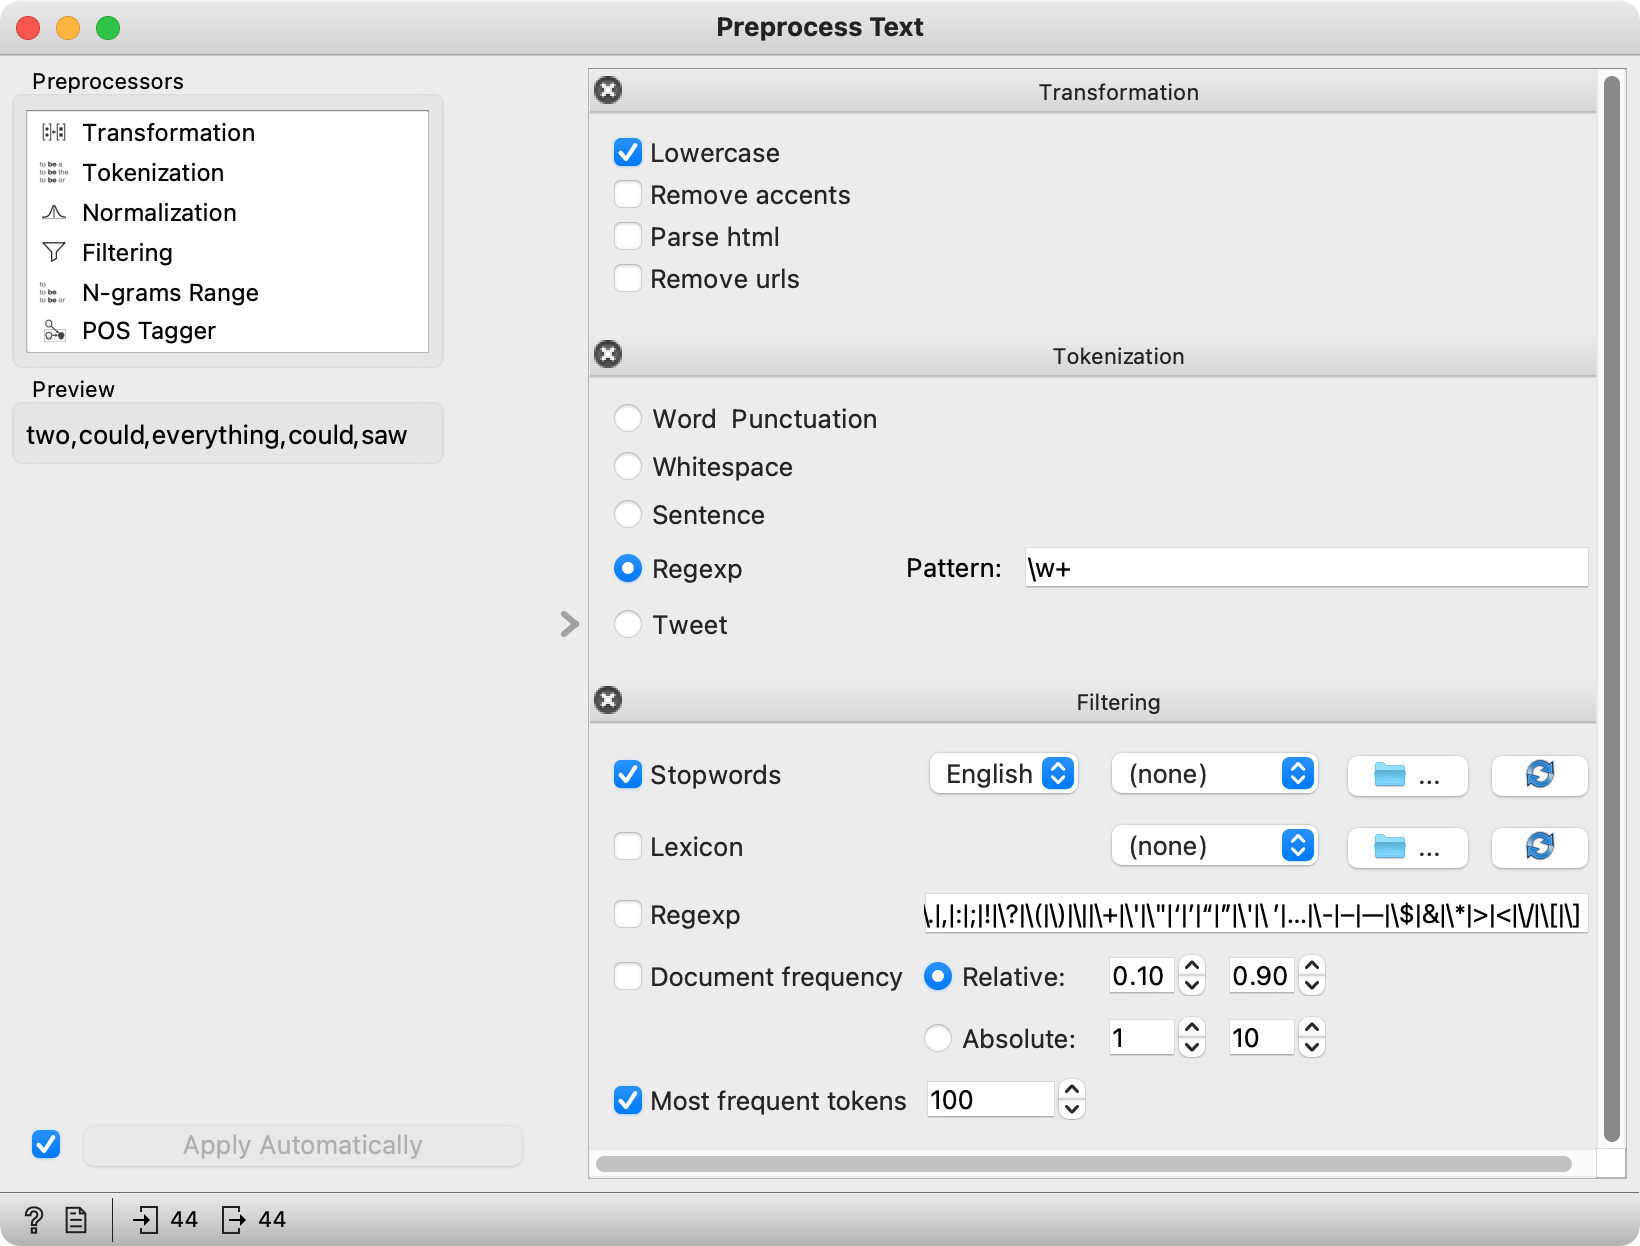
\includegraphics[width=\linewidth]{preprocess-text.png}
    \caption{$\;$}
\end{figure*}

Now pass the data to \widget{Corpus to Network}. With this widget, we will generate the graph. If we are generating network where nodes are documents, then we need to set a single parameter, namely the threshold. This is similar to the similarity threshold in \widget{Network from Distances}. \emph{Threshold} will define how many words the documents have to share for them to have a connecting edge. In our case, we will set the threshold quite high - two documents have to share at least 50 words to be connected with an edge.

\begin{figure}[h]
    \centering
    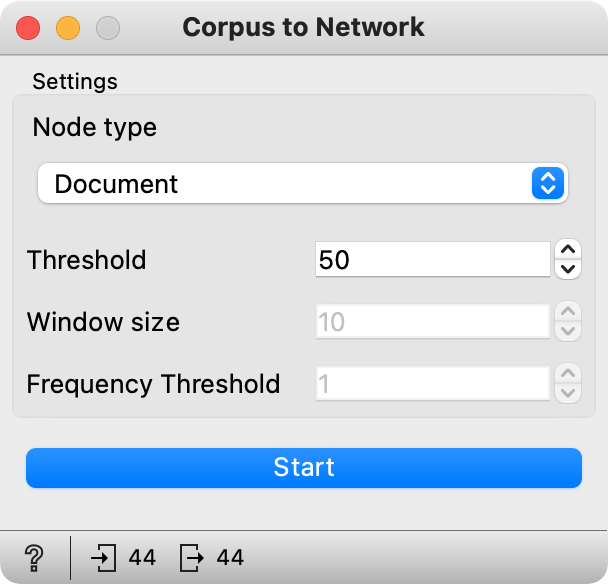
\includegraphics[scale=0.6]{corpus-to-network.png}
    \caption{$\;$}
\end{figure}

Let us observe the end result in \widget{Network Explorer}. Seem like Tales of Magic are well-connected, even with some Animal Tale, while certain Animal Tales are quite distinct and don't share as many words with the other tales.

\begin{figure*}[h]
    \centering
    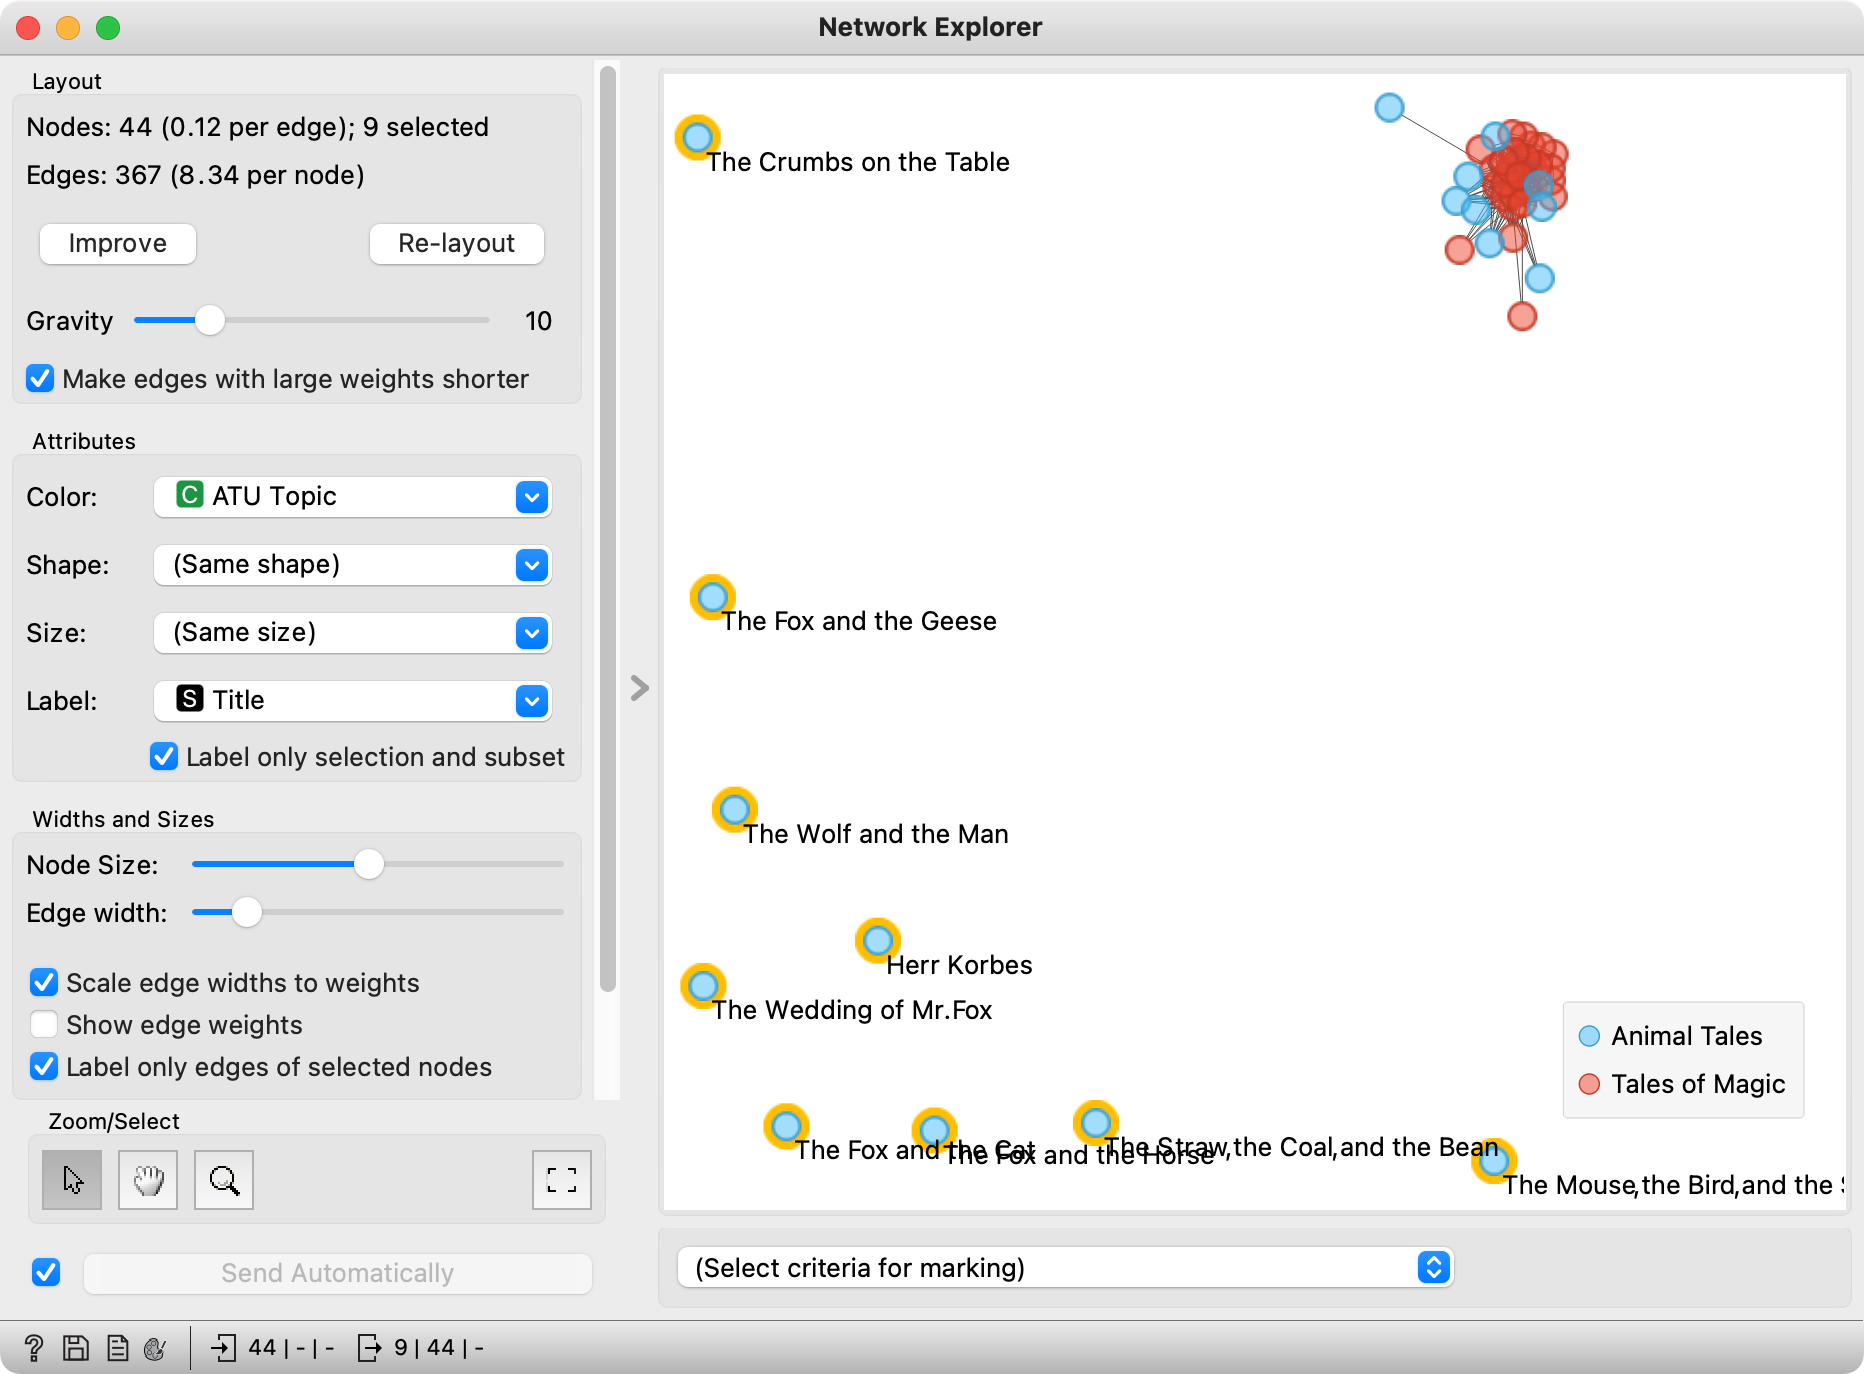
\includegraphics[width=0.9\linewidth]{network-explorer.png}
    \caption{$\;$}
\end{figure*}

A task for the reader: play with the threshold and observe how the graph changes. Does a lower threshold results in a more or less connected graph? What happens if words are used as Node types in \widget{Corpus to Network}? What does such a graph show?

\begin{figure}[h]
    \centering
    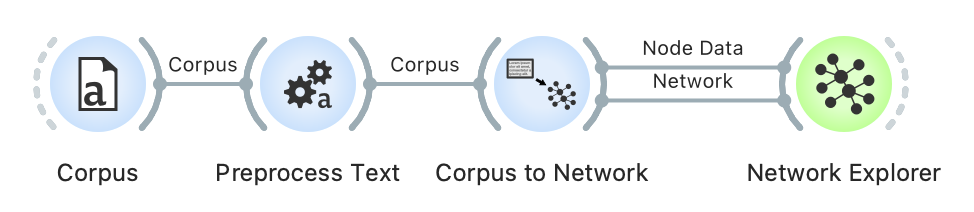
\includegraphics[width=\linewidth]{workflow.png}
    \caption{$\;$}
\end{figure}
